\section{Introduction}
\label{sec:Introduction}

Construction industry is becoming increasingly data intensive with the growing use of
information and communication technology in all phases of a building life-cycle. 
In the future, buildings will act as hubs of a wide variety of real-time and accumulated data about
spaces, indoor locations, indoor routes, assets, people, sensors, materials, equipment, connections
to surrounding networks (traffic, infrastructure, communication), detected issues, and activities in the building.

Currently, a huge amount of basic design information about buildings are produced  
using modern Building Information Modeling (BIM) tools. There is a widely adopted standard, 
IFC (Industry Foundation Classes) that provides a common representation of building designs developed in different design disciplines: architecture, structural engineering,
MEP engineering, and so on. Nowadays, the IFC standard is supported by all major BIM
vendors; their BIM tools can export building models as IFC files that can be exchanged with other
parties.

The BIM models could provide a natural framework to organize and manage information gathered from other sources. However, a big obstacle to that is the difficulty to access and utilize BIM models. 
In the realm of IFC the sharing of building models is based on point-to-point file exchange which 
requires repeated manual work from designers. Information cannot be used in an online, granular, and interlinked manner, which provides a poor basis for open utilization of building information and the emergence of new, innovative applications.

To make building information more readily accessible, we have developed a \emph{WebIFC converter} to derive an OWL ontology from the IFC schema (\emph{ifcOWL}), and RDF datasets from IFC files (\emph{ifcRDF}). The ifcOWL ontology is used to classify concepts, characterize possible relationships, and define constraints in ifcRDF datasets which replicate the content of original IFC data files. All terms defined in the ifcOWL ontology must therefore be based on the corresponding constructs in the original IFC schema. The conversion from IFC data files to RDF is straightforward and can be done without information loss.

Ideally, there should also be just one ifcOWL ontology for each version of the IFC schema (Fig. \ref{fig:ifcOWL-layers}, a). However, the conversion from the EXPRESS data definition language (that is used to specify the IFC schema) to OWL can be done in several different ways for the following reasons. Firstly, there is a \emph{mismatch} between the modeling constructs between EXPRESS and OWL. Secondly, for most practical purposes, the IFC data can be considered \emph{valid and consistent} with respect to the schema, since the IFC models are exported from BIM tools with certified converters. Thirdly, as the master data of the design models will remain in the native formats of the BIM tools and evolves over time, the icfRDF can in practice only be used in a \emph{read-only} fashion. Fourthly, the conversion of all possible IFC schema information will lead into a \emph{extensive} OWL ontology that mostly contains information not needed in practical applications or use cases.

Consequently, we have converted the IFC schema into a \emph{flexible, multilayer ifcOWL ontology}. Different representational constructs are introduced at different levels. The ifcRDF is compatible with any of the layers; different layers just provide different amounts of type information that can be used with RDF. 

\begin{figure}[h]
\centering
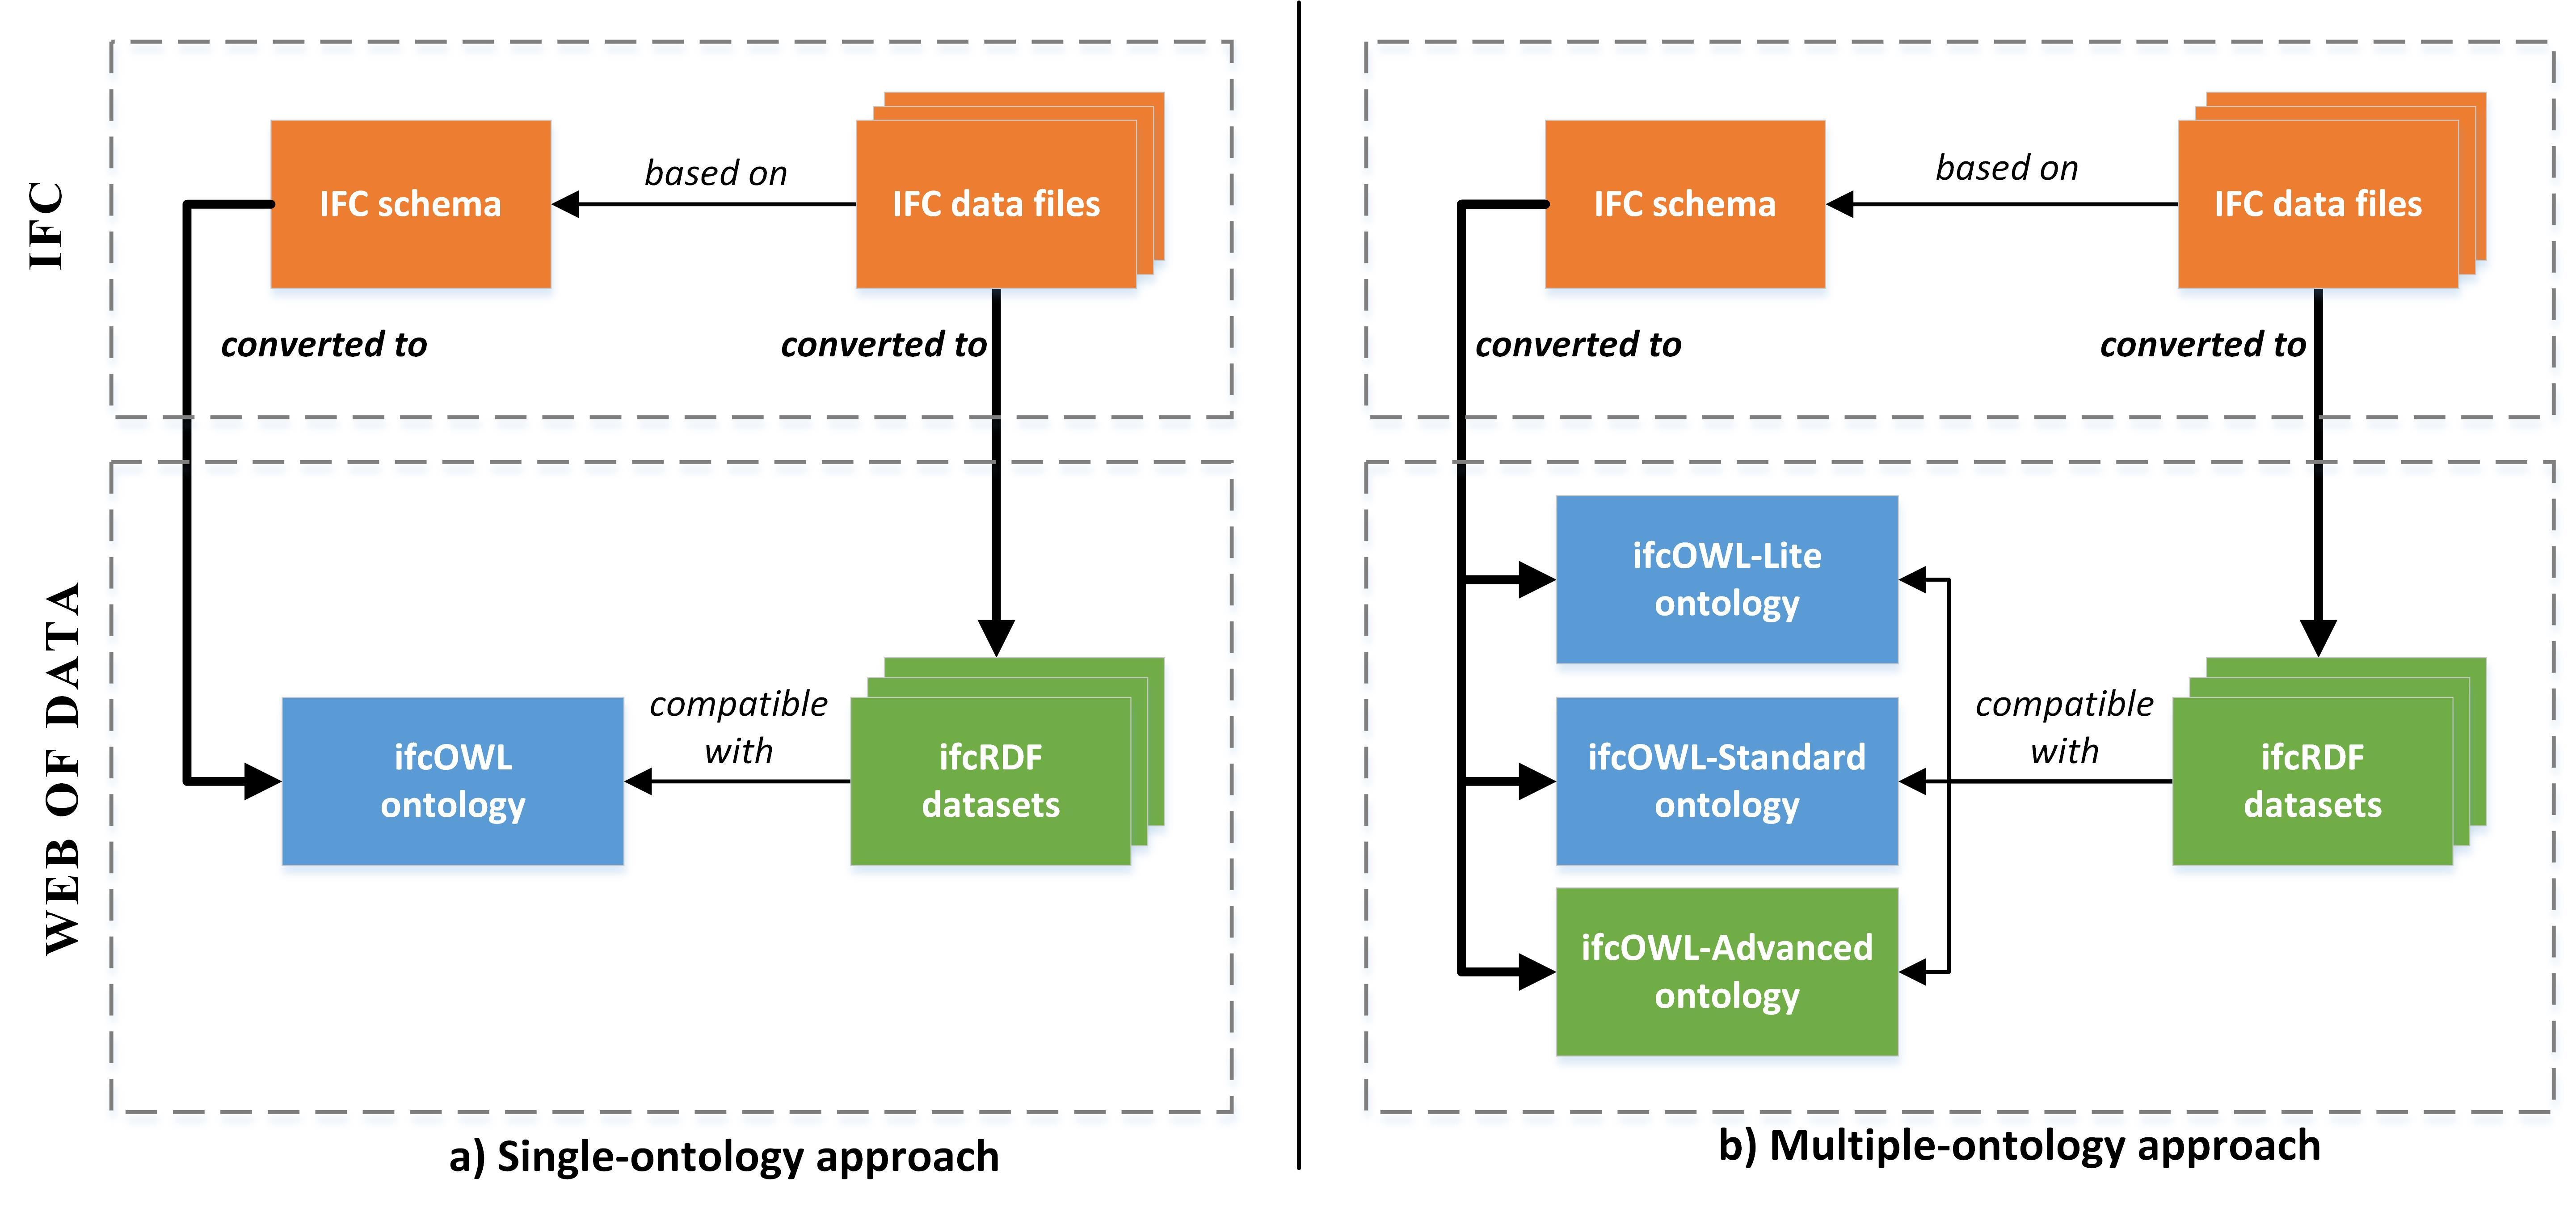
\includegraphics{images/ifcOWL-approaches.jpg}
\caption{Two approaches of creating and using ifcOWL ontology}
\label{fig:ifcOWL-layers}
\end{figure}

Different levels of details of the ifcOWL ontology are the following:

\begin{enumerate}
\item
    \textbf{ifcOWL-Lite} (compatible with OWL 2 EL, OWL 2 QL, OWL 2 RL)
    \begin{itemize}
        \item Schema meta data
        \item All type definitions and hierarchies
        \item All entity type properties (names and range types)
    \end{itemize}
\item
    \textbf{ifcOWL-Standard} (compatible with OWL 2 RL)
    \begin{itemize}
        \item Schema meta data
        \item All entity type keys
        \item All entity type inverse properties
    \end{itemize}
\item
    \textbf{ifcOWL-Advanced} (compatible with OWL 2 RL)
    \begin{itemize}
        \item All properties' cardinality constraints
        \item All list types' cardinality constraints
    \end{itemize}
\end{enumerate}

Since all ifcRDF datasets are compatible with all layers of the ifcOWL ontology (Fig. \ref{fig:ifcOWL-layers}, b), a user can choose the best one based on the requirements of the concrete use case and tools. For instance, many Linked Data applications that need to query entity properties, extract the type hierarchy, or convert ifcRDF datasets back to object-oriented data models it is sufficient to use the \textbf{ifcOWL-Lite} ontology. In case of reasoning about data that includes inverse properties, it is recommended to use \textbf{ifcOWL-Standard} ontology. If an RDF dataset needs to be modified and data validated using type and cardinality constraints, \textbf{ifcOWL-Advanced} ontology is the right choice.


% \begin{figure}
% \centering
% %\def\svgwidth{\textwidth}
% \def\svgscale{1}
% \input{images/image.pdf_tex}
% %{\includesvg{images/test-2}}
% %\includegraphics[width=0.75\textwidth]{images/ifcOWL-multilayer-2.png}
% \caption{A multilayer ifcOWL ontology}
% \label{fig:ifcOWL-multilayered}
% \end{figure}